% \documentclass[letterpaper, 10pt, conference]{ieeeconf}

\documentclass[graybox]{svmult}


\let\proof\relax
\let\endproof\relax

\usepackage{mathptmx}
\usepackage{eucal}
\usepackage{helvet}
\usepackage{courier}
\usepackage{makeidx}
\usepackage{graphicx}
\usepackage{multicol}
\usepackage[bottom]{footmisc}
\usepackage{amsmath, amssymb}
\usepackage{url}
\usepackage{float}
\usepackage{relsize}
\usepackage{algorithm}
\usepackage{fancyvrb}
\usepackage[noend]{algorithmic}
\usepackage{subfiles}
\usepackage{titlecaps}
\usepackage{fancyhdr}
\usepackage{amsthm}

\graphicspath{{resources/}}

\renewcommand{\thefootnote}{\fnsymbol{footnote}}
\renewcommand{\algorithmicrequire}{\textbf{Input:}}
\renewcommand{\algorithmicensure}{\textbf{Output:}}

\newcommand{\tab}[1]{\hspace{.2\textwidth}\rlap{#1}}
\newcommand{\itab}[1]{\hspace{0em}\rlap{#1}}
\renewcommand{\thefootnote}{\fnsymbol{footnote}}
\newcommand{\Acronym}[1]{\ensuremath{{{\texttt{#1}}}}}
\newcommand{\Symbol}[1]{\ensuremath{\mathcal{#1}}}
\newcommand{\Function}[1]{\ensuremath{{\textsc{#1}}}}
\newcommand{\Area}[0]{\ensuremath{{\textsc{Area}}}}
\newcommand{\Constant}[1]{\ensuremath{{\texttt{#1}}}}
\newcommand{\Var}[1]{\ensuremath{{{\textsl{#1}}}}}
\newcommand{\rB}[0]{\ensuremath{{{\mathcal{B'}}}}}
\newcommand{\B}[0]{\ensuremath{{{\mathcal{B}}}}}
\newcommand{\False}{\Constant{false}}
\newcommand{\True}{\Constant{true}}
\newcommand{\Null}{\Constant{null}}
\newcommand{\dif}{\ensuremath{{\mathrm{d}}}}
\newcommand{\where}{\ensuremath{{\textbf{ where }}}}
\newcommand{\Name}{\Acronym{Dodger}}
\newcommand{\Revision}[1]{\textcolor{red}{#1}}
\newcommand{\R}{\ensuremath{\mathbb{R}}}
\newcommand{\Traj}{\ensuremath{\zeta}}
\newcommand{\Tree}{\Symbol{T}}
\newcommand{\pair}[1]{\ensuremath{\langle#1\rangle}}
\newcommand{\argmin}[1]{\underset{#1}{\operatorname{arg}\,\operatorname{min}}\;}
\newcommand{\argmax}[1]{\underset{#1}{\operatorname{arg}\,\operatorname{max}}\;}
\newcommand{\mychange}[1]{\textcolor{red}{#1}}

% \newtheorem{theorem}{Theorem}
% \newtheorem{lemma}{Lemma}
% \newtheorem{corollary}{Corollary}
% \newtheorem{definition}{Definition}
% \newtheorem{problem}{Problem}

\makeindex

\begin{document}

\title*{Foresight: Remote Sensing For Autonomous Vehicles Using a Small
Unmanned Aerial Vehicle}

\titlerunning{Foresight: Remote Sensing For Autonomous Vehicles}

\author{Alex Wallar \and Brandon Araki \and Javier Alonso-Mora \and Raphael Chang
\and Daniela Rus}

\institute{Alex Wallar \at Massachusetts Institute of Technology, \email{wallar@mit.edu}}

\maketitle

\begin{abstract}
% !TEX root = ../foresight.tex
\begin{abstract}
This method presents a method augment what a self-driving car can see.
- Occlusions limit the field of view of the car
- A small UAV can fly to explore those blind spots and prevent accidents
- Informative / exploration planning algorithm for the UAV
- Open source communication framework for multi-robot systems
- Experiments with real data captured from our car 
\end{abstract}
\end{abstract}

% !TEX root = ../foresight.tex

\section{Introduction}

Introduction: Lots of accidents due to not seeing what's going on. For example a pedestrian or a biker behind a car.

This method presents a method augment what a self-driving car can see.
- Occlusions limit the field of view of the car
- A small UAV can fly to explore those blind spots and prevent accidents
- Informative / exploration planning algorithm for the UAV
- Open source communication framework for multi-robot systems
- Experiments with real data captured from our car 

\subsection{Related works}

In autonomous cars

In mutli-robot mapping

In informative planning and exploration

\subsection{Contribution}

\begin{itemize}
\item
Method for informative sensing
\item
Open source communication framework
\end{itemize}

We validate our approach with data collected with our self-driving vehicle and a small UAV.

% !TEX root = ../foresight.tex

\subsection{Method overview}

We consider two vehicles.
\begin{itemize}
\item
A ground vehicle, i.e. the car, which can create a local map of the environment, localize with respect to it and autonomously navigate \cite{Add citation to Felix's IV paper}. We utilize a 2D grid map to represent the free space and obstacles seen by the car. In particular, our vehicle is equipped with a 2D LIDAR. 
\item
A lightweight companion quadrotor \footnote{We use a Parrot Bebop 2} equipped with a front facing camera. The drone is able to fly autonomously to/from the ground vehicle and detect obstacles that were originally occluded for the ground vehicle.
\end{itemize}

Given a laser scan from the ground vehicle, our objective is to:
a) determine which areas of the environment are occluded to ground vehicle,
b) compute a safe path for the aerial vehicle to observe the occluded areas, and
c) detect unseen obstacles, such as pedestrians, and report them back to the ground vehicle.

% Our problem is two pronged. First we need to be able to accurately localize the
% quadrotor in the same reference frame as the vehicle. Second, we need to
% determine which areas of the environment are occluded to ground vehicle, and
% compute a safe path that leads the quadrotor to view these regions.

% % \begin{problem}
% %
% %     Given a laser scan from the ground vehicle, compute a path the maximizes
% %     the occluded area observed by the quadrotor for a given time horizon.
% % \end{problem}
%
% We used a Parrot Bebop 2 as the quadcopter. It is equipped with a camera, and
% velocity and altitude measurements can be read from its SDK at a rate of 5 Hz.
% The Bebop uses a software gimbal to stabilize the camera image.
%
% The inputs to the Bebop are roll angle $\phi$, pitch angle $\theta$, 
% yaw rate $\omega$, and z velocity $\dot{z}$. We use
% PID controllers to control the inputs.
%
% $$ u = [\phi, \theta, \omega, \dot{z}] $$

%\subsection{Method overview}

To accurately localize the quadrotor relative to the ground vehicle, we equip the ground vehicle with several Ultra-wideband radios. In the quadrotor, we fuse, via an Unscented Kalman filter (UKF) relative information from a UWB radio with odometry estimates from a down facing optical flow sensor and an onboard IMU.
% We use an unscented Kalman filter to fuse these
% measurements and produce an estimate of quads 3D position relative to the
% ground vehicle.
Our algorithm operates directly on the laser scan from the ground vehicle to find occluded
regions.
We then employ an anytime sampling-based algorithm to compute a collision free path for the drone
that maximizes the occluded area viewed by the quadrotor.
% and builds a search tree from the quadrotor's current configuration
% towards these regions. The search terminates when a timeout has expired and
% returns the path that currently maximizes the occluded area viewed by the
% quadrotor.
To detect obstacles within the occluded areas, we employ a real-time object detecting convolutional neural network~\cite{yolo}, which is able to classify and locate objects, such as pedestrians, cars, bicycles, in monocular images. These obstacles are then reported back to the ground vehicle.



Thanks to the differential flatness of quadrotor vehicles, we model our quadrotor by its position $\bm{p}$ and yaw orientation $\psi$, measured in the car's body frame. We therefore describe the state of the quadrotor as

$$
    x = [\bm{p}, \psi] \in \R^4
$$


\ja{Can you add here a high-level algorithm? Car maps -> compute blind spots -> plan path -> navigate to bind spots -> detect occluded obstacles -> loop}


% !TEX root = ../foresight.tex

\section{Relative pose localization}

From each UWB tag we receive a range measurement $r_i$ in its own frame. 
From the quadrotor we receive velocity measurements $\bm{v}$, a yaw reading $\psi_q$,
and an altitude measurement $z_a$ in an ENU-aligned world frame. The frames and relative
transforms of our system are visualized in Fig.~\ref{fig:frames}.
Given $n$ UWBs, we define the measurement vector as $z = [r_1, \dots, r_n, \bm{v}, z_a, \psi_q] \in \R^{n+5}$

%We use 6 ultra-wideband radios and the Bebop's onboard odometry measurements
%to estimate the relative position of the quadcopter with respect to the car with an
%accuracy of 13 cm. The 6 UWBs were positioned as far apart as possible on the
%car while still maintaining line of sight with the quadcopter when the
%quadcopter is positioned in front of the car. The transform from a set base position
%on the car to each UWB was then measured. These transforms allow us to
%calculate the distance between each UWB and the estimated state of the quadcopter.


Yaw orientation is calibrated at the start by lining up the quadrotor along the car's x-axis
and measuring the yaw offset $\psi_{\text{off}}$ between the car and the quadrotor.
The yaw of the quadrotor is then given by $\psi = \psi_q - \psi_{\text{off}}$

One challenge we encountered in estimating the 3D position of the quadrotor was that
the distance measurements from the UWBs showed larger errors when the UWB on the quadrotor was out of their plane.
We therefore first estimate $\bm{\hat{p}^{\text{odom}}}$ using only use the quadrotor's onboard 
odometry readings $\bm{v}$ and $z_a$ as the inputs to a UKF. We then use the estimated
height, $\bm{\hat{p}_z^{\text{odom}}}$ with the UWB range
measurements $r_i$ to estimate the quadrotor's x-y position, $\bm{\hat{p}^{xy}}$.
We do this by first projecting each $r_i$ onto the plane of the estimated height of the quadrotor:

$$
   r_i^{\text{proj}} = \sqrt{r_i^2 - (\bm{\hat{p}_z^{\text{odom}}})^2}
$$

We then find $\bm{\hat{p}^{xy}}$ by solving the nonlinear least squares optimization

\begin{align*} 
    h(\bm{\hat{p}^{xy}}) = \min_{{\bm{\hat{p}^{xy}}}} \sum_{i=1}^{n} ((r_{i}^{\text{proj}})^2 - \lVert \bm{\hat{p}^{xy}} - \bm{t_i^{xy}}\rVert^2)^2
\end{align*}

% with the Jacobian \ja{with respect to what? P? If so, I think it is not correct. Please check.}
%
% $$
%     H(\bm{\hat{p}^{xy}}) = \frac{dh(\bm{\hat{p}^{xy}})}{d\bm{\hat{p}^{xy}}} = \sum_{i=1}^{n} 4((r_i^{\text{proj}})^2 - \lVert \bm{\hat{p}^{xy}} - \bm{t_i^{xy}} \rVert^2)[(\bm{t_i^{x}} - \bm{\hat{p}^{x}}), (\bm{t_i^{y}} - \bm{\hat{p}^{y}})]
% $$

We then define the 3D position estimate to be $\bm{\hat{p}^{ls}} = [\bm{\hat{p}^{xy}}, \hat{z}]$. Next, we combine $\bm{\hat{p}^{ls}}$ and $\bm{\hat{p}^{\text{odom}}}$ in a second UKF to find a final position estimate $\bm{\hat{p}}$. Thus the final state estimate is $\hat{x} = [\bm{\hat{p}}, \psi]$.


\begin{figure}[tb!]
  \centering
    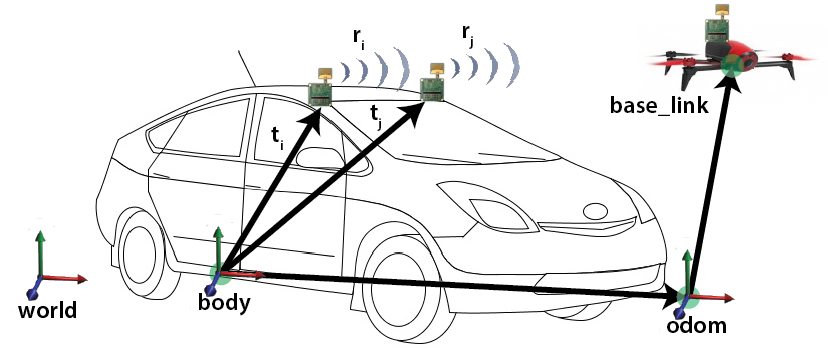
\includegraphics[width=0.7\textwidth]{foresight_frames}
  \caption{The frames and measurements of our system.}
  \label{fig:frames}
\end{figure}









% !TEX root = ../foresight.tex

\section{Planning For Exploration}

Planning a path to observe the blind spots of an autonomous car is broken into
following steps. First, using the 2D laser scan from the car, the bounding
polygon is computed. This polygon represents the known free space where the
quadrotor can travel. The laser scan is also used to determine regions in space
where that the car is not able to sense. These regions are called blind
regions. Using these blind regions and the bounding polygon, a path is computed
for the quadrotor that maximizes the observed area of the blind regions while
staying within the bounding polygon. The path is computed for a given time
horizon.

The remainder of this section is structured as follows; Sec.~\ref{sec:poly}
introduces the our formal definition of a laser scan and describes how the
bounding polygon is found, Sec.~\ref{sec:blindregions} describes how the blind
regions are computed from the laser scan, and Sec.~\ref{sec:planner} describes
and analyzes the algorithm we developed for computing the exploratory path.

\begin{figure}[ht]

    \centering

    \begin{subfigure}[t]{0.44\textwidth}
        \centering
        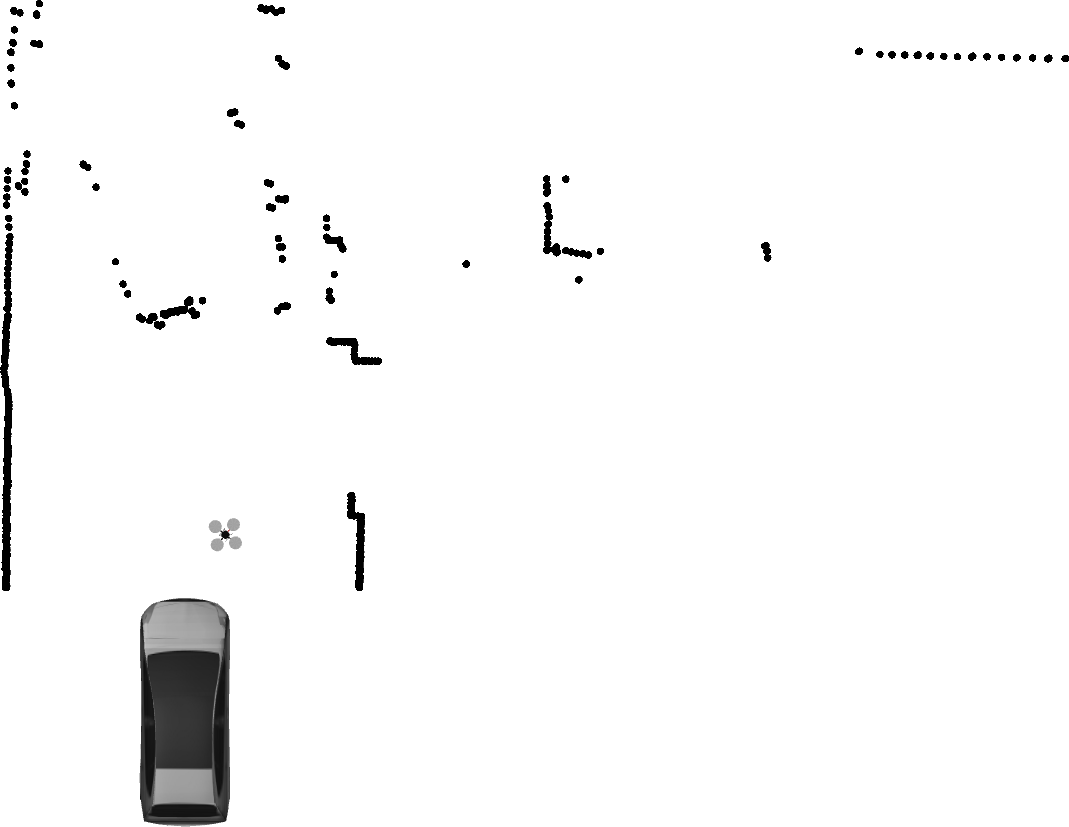
\includegraphics[width=1\linewidth]{01laser}
        \caption{}
        \label{fig:01laser}
    \end{subfigure}
    ~
    \begin{subfigure}[t]{0.44\textwidth}
        \centering
        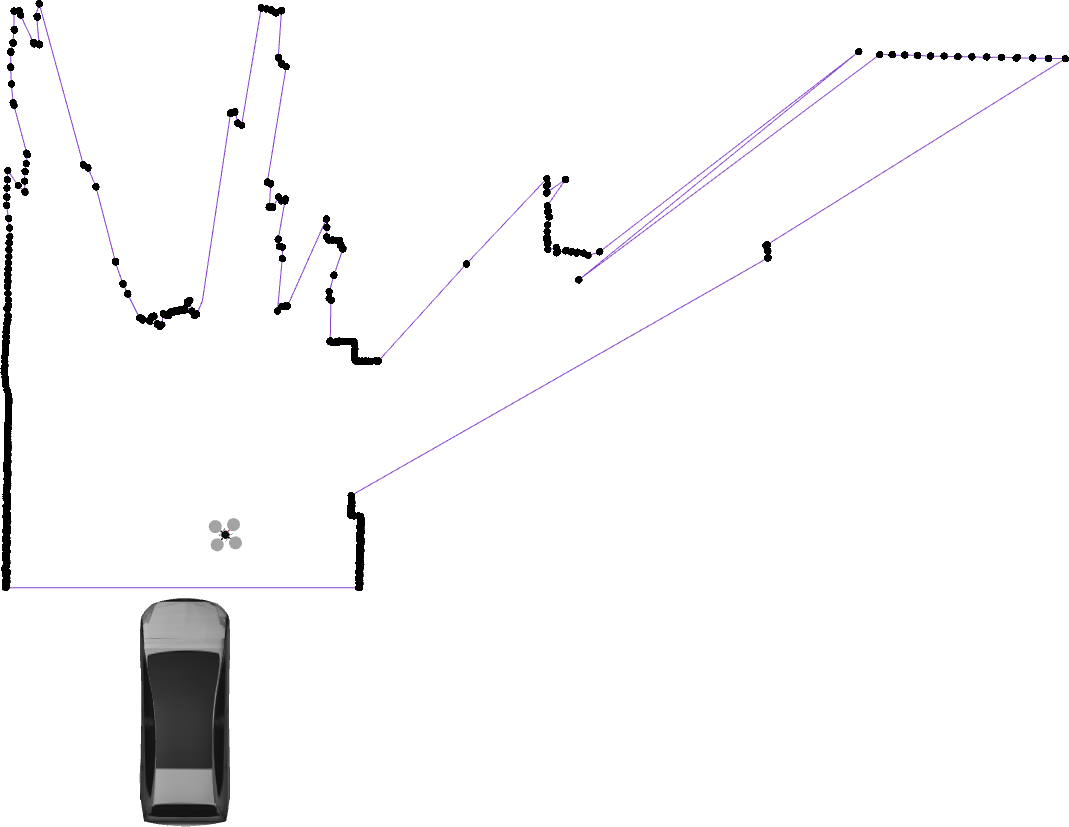
\includegraphics[width=1\linewidth]{02polygon}
        \caption{}
        \label{fig:02polygon}
    \end{subfigure}
    ~
    \begin{subfigure}[t]{0.44\textwidth}
        \centering
        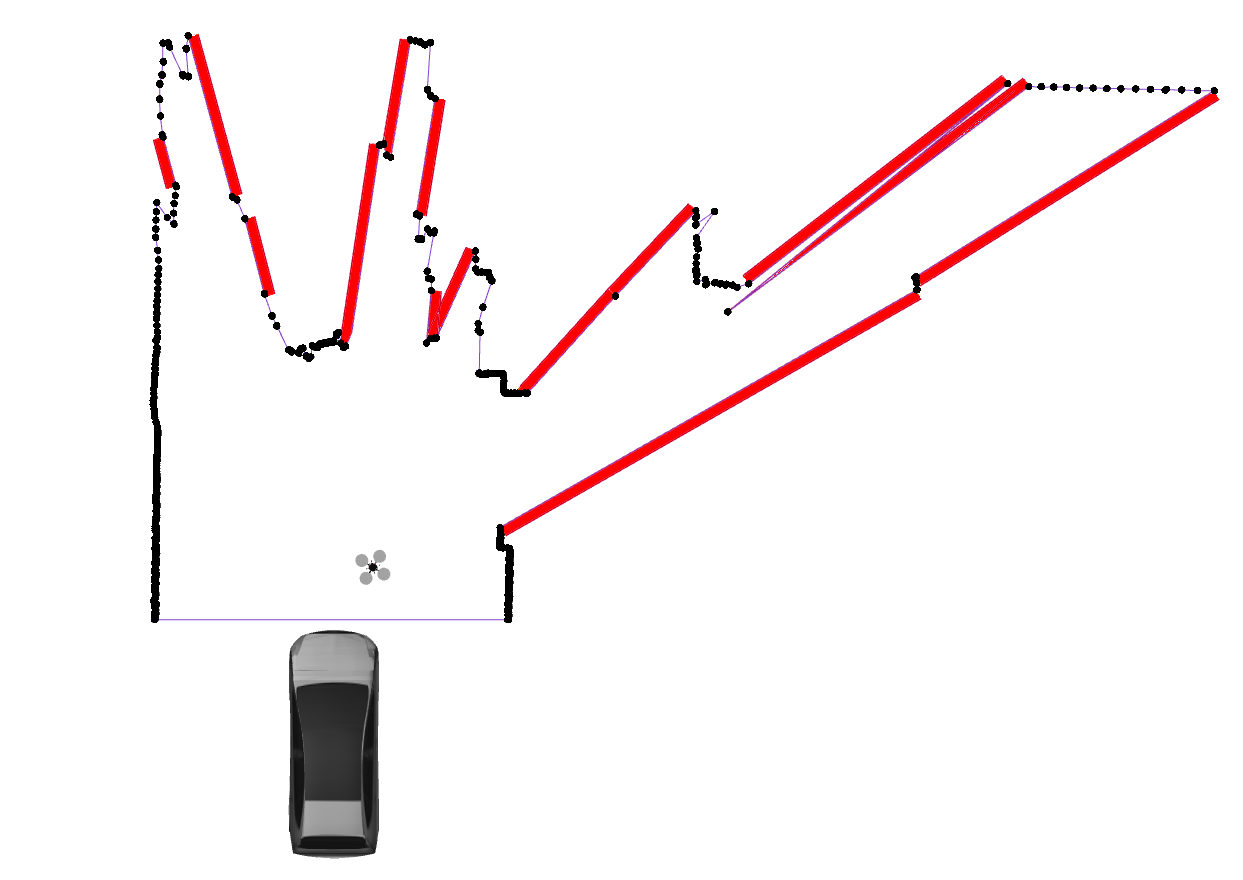
\includegraphics[width=1\linewidth]{03blindregions}
        \caption{}
        \label{fig:03blindregions}
    \end{subfigure}
    ~
    \begin{subfigure}[t]{0.44\textwidth}
        \centering
        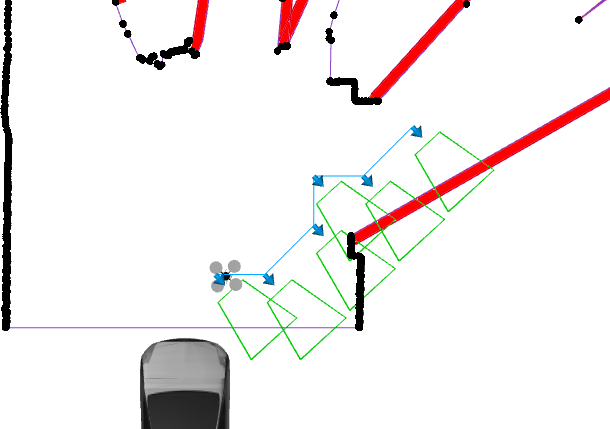
\includegraphics[width=1\linewidth]{04planner-small}
        \caption{}
        \label{fig:04planner-small}
    \end{subfigure}

    \caption{Plots showing the four stages of the planner. Fig. (a) shows the
    points from the laser scan. Fig. (b) shows bounding polygon created from
the laser scan. Fig. (c) shows the regions occluded to the vehicle in red and
Fig. (d) shows the initial plan for the quadrotor to view some of these blind
regions.}

    \label{fig:planner-stages}

\end{figure}

\subsection{Finding the Bounding Polygon}

\label{sec:poly}

The bounding polygon computed using a scan from the 2D LiDAR sensor on the car
is used as a conservative representation of the free space in which the
quadrotor can travel. Below we provide a formal definition of a laser scan that
is used in the rest of the paper.

\begin{definition}

    A laser scan is a sequence of points, $L = \{\mathbf{c} + r_i \cdot [\cos
    \theta_i, \sin \theta_i] ^ T : \theta_{\min} \leq \theta_i \leq
    \theta_{\max} \} \subset \R^2$, where $\mathbf{c}$ is the 2D position of
    the LiDAR sensor, $r_i$ is the distance from the sensor to the closest
    obstruction in the $\theta_i$ direction, and
    $[\theta_{\min}$, $\theta_{\max}]$ is the angular range of the sensor.

\end{definition}

From the laser scan, we compute a bounding polygon. The bounding
polygon is defined as the minimum area simple polygon that contains all the
points in the laser scan. Since the laser scan data is ordered by $\theta_i$
from $\theta_{\min}$ to $\theta_{\max}$, the bounding polygon can be
constructed in one pass with the vertex sequence $\{\mathbf{c}\} \cup L \cup
\{\mathbf{c}\}$. Fig.~\ref{fig:02polygon} shows an example of laser scan
data and the corresponding bounding polygon.

\subsection{Determining the Blind Regions}

\label{sec:blindregions}

Using the laser scan data, we can determine which areas in the environment the
car is unable to sense. We call these areas blind regions. The blind region,
$\B$, is the set of points contained within a rectangle with a vertex sequence
$\{L_i, L_i + k \cdot \hat{L}_{i, i + 1}, L_{i + 1} + k \cdot \hat{L}_{i, i +
1}, L_{i + 1}, L_i\}$ where $\hat{L}_{i, i + 1}$ is the unit normal for the
vector between points $L_i$ and $L_{i + 1}$ that points away from the bounding
polygon and $k$ is a tuning parameter that contributes to the area of the blind
region. In practice we only care for blind regions where $||L_i - L_{i + 1}||_2
> \delta$ where $\delta$ is a tuning parameter because the laser scan consists
of a finite number of points with a known angular distance. We will use $\B$ to
denote the set of all such regions.  Fig.~\ref{fig:03blindregions} shows an
example of blind regions in found in a found from a laser scan.

% maybe can change the name of this section
\subsection{Computing the Exploratory Path}

\label{sec:planner}

Using the blind regions, current configuration of the quadrotor, and the
bounding polygon, we present an anytime algorithm that computes a collision
free path for the quadrotor that maximizes the total observed area of the blind
regions within a given time horizon. The algorithm builds a search tree
starting from the current configuration of the quadrotor. It expands leaf nodes
in descending order of total observed blind region area and only adds new leaf
nodes to the search that are contained within the bounding polygon. When a
collision free neighbour is propagated, the orientation, $\theta^*(x, \B)$,
that maximizes the area of the remaining blind region, $\B$, viewed at that
configuration, $x$, is also added to the search tree. Below we formally define
this orientation.

\begin{definition}

    Let $\psi(x, \theta, \B)$ be the set of points visible by the quadrotor at
    position $x \in \R^3$ with orientation $\theta$. Let $\theta^*(x, \B) =
    \argmax{0 < \theta \leq 2\pi} \psi(x, \theta, \B)$. For convenience, we
    define $\psi^*(x, \B) = \psi(x, \theta^*(x, \B), \B)$.
    % \ja{What are the visiblie points?}

\end{definition}

As the quadrotor follows the path, the planner is constantly replanning. To
avoid oscillating between candidate paths, the quadrotor only follows a new
path if its current path is no longer collision free or if the new path has a
larger objective value. % \ja{ADD caption to algorithm and figure!}

\begin{algorithm}[h!]
    \caption{Path planning for remote sensing UAV (looking around the corner)}
    \algorithmicrequire{\begin{itemize}
            \item $x_0$: The initial position of the robot,
                $\B$: The blind region, $\Poly$: The bounding polygon
        \end{itemize}}
    \algorithmicensure{\begin{itemize}
            \item $\Pi \subset \R^3 \times [0, 2\pi]$: A sequence of 3D positions
                and orientations representing the path
        \end{itemize}}
    \label{algo:find_path}
    \begin{algorithmic}[1]
        \setcounter{ALC@line}{0}
        % \vspace*{1mm}

        \STATE $Q \leftarrow \{(x_0, \theta^*(x_0, \B),
            \B \, \backslash \, \psi^*(x_0, \B))\}$
        \WHILE{$|Q| > 0$}

        \STATE $(x, \theta, \rB) \leftarrow \argmin{\rB \in Q} \Area(\rB)$

            \IF{$\Function{SearchTimeoutExpired}()$}
                \STATE $\Pi \leftarrow \{\}$
                \WHILE{$\Function{HasParent}(x, \theta)$}
                    \STATE $\Pi \leftarrow \Pi \cup \{x\}$
                    \STATE $(x, \theta) \leftarrow \Function{Parent}(x, \theta)$
                \ENDWHILE
                \RETURN $\Pi$
            \ENDIF
            \FORALL{$x' \in \Function{CollisionFreeNeighbours}(x, \Poly)$}
            \STATE $\theta' \leftarrow \theta^*(x', \rB)$
            \STATE $Q \leftarrow Q \cup \{(x', \theta', \rB \, \backslash \,
                    \psi^*(x', \rB))\}$
                \STATE $\Function{Parent}(x', \theta') \leftarrow (x, \theta)$
            \ENDFOR
            \STATE $Q \leftarrow Q \, \backslash \, \{(x, \theta', \rB)\}$
        \ENDWHILE
        \RETURN $\{\}$

    \end{algorithmic}
\end{algorithm}

At the start of Algo.~\ref{algo:find_path}, we initialize a priority queue that
is used to store the leaf nodes of the search tree. Each node is comprised of
the position of the quadrotor, $x \in \R^3$, the orientation of the quadrotor
on the Z-axis, $\theta \in [0, 2\pi]$, and the remaining blind region, $\B$,
that is left unobserved after the quadrotor reaches $x$ with orientation
$\theta$. Until the search timeout has expired, collision free neighbours of
$x$ are added to the search along with their maximizing orientation and
remaining unobserved blind regions.  Once the search has expired, the path,
$\Pi$ comprised of 3D positions and orientations, that was able to view the
largest cumulative blind region area starting from $x_0$ is returned.
Fig.~\ref{fig:04planner-small} shows an example of a path being computed to
view the blind regions.

\subsection{Autonomous Landing}

To enable autonomous landing, the quadrotor tries to maintain a static position
relative to the car as it drives towards a parking spot. Once the vehicle has
stopped, the quadrotor moves directly above the landing platform and proceeds
to land on the platform.


% !TEX root = ../foresight.tex

\section{Results}

In this section we provide experimental results that validate our approach. A video accompanies this submission and is available at \ja{add link to website}.

\subsection{Localization Accuracy}

We tested our localization framework by emulating the car's ultra-wideband
sensor configuration inside a motion capture system. We placed motion capture
markers on the quadrotor and on each ultra-wideband sensor. This allowed us to
obtain the absolute position of the quadrotor and UWBs in the same coordinate
frame. We then flew the quadrotor inside the motion capture system and recorded
its predicted position determined by our localization and absolute position
using the motion capture markers. The average error in our localization was
13.7 cm, or 35.9\% the length of the quadrotor. Fig.~\ref{fig:localization}
shows how our localization compares to the ground truth. The green and red
lines respectively show the ground truth and predicted positions of the
quadrotor.\ja{How come it is worse than the reported errors in the UWB paper that we are citing?}

\begin{figure}

    \centering

    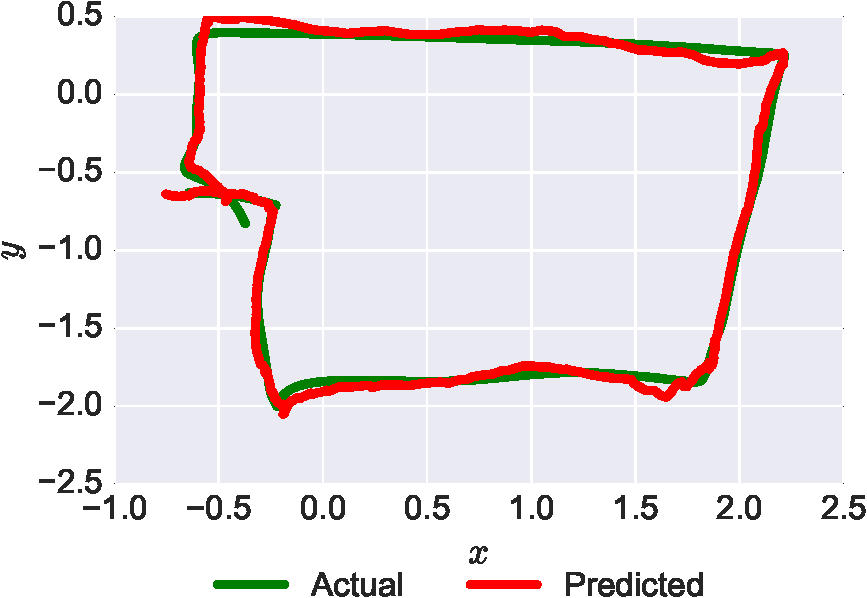
\includegraphics[width=0.7\linewidth]{localization}

    \caption{Comparison of our localization method with respect to
    ground truth. Ground truth was supplied by a motion capture system.}

    \label{fig:localization}

\end{figure}

\subsection{Experimental Setup}

For our experiments, we used a Toyota Prius with a SICK LMS1xx mounted on the
front of the car and six Decawave TREK1000 ultra-wideband radios mounted on the
roof and front bumper of the car. A platform for the quadrotor to take off and
land is attached to the front bumper of the Prius. We used a Parrot Bebop 2
quadrotor with a Decawave TREK1000 mounted on the battery.  Fig.~\ref{fig:car}
shows the Toyota Prius and modified Bebop 2 quadrotor used in the experiments.

\begin{figure}[h!]

    \centering

    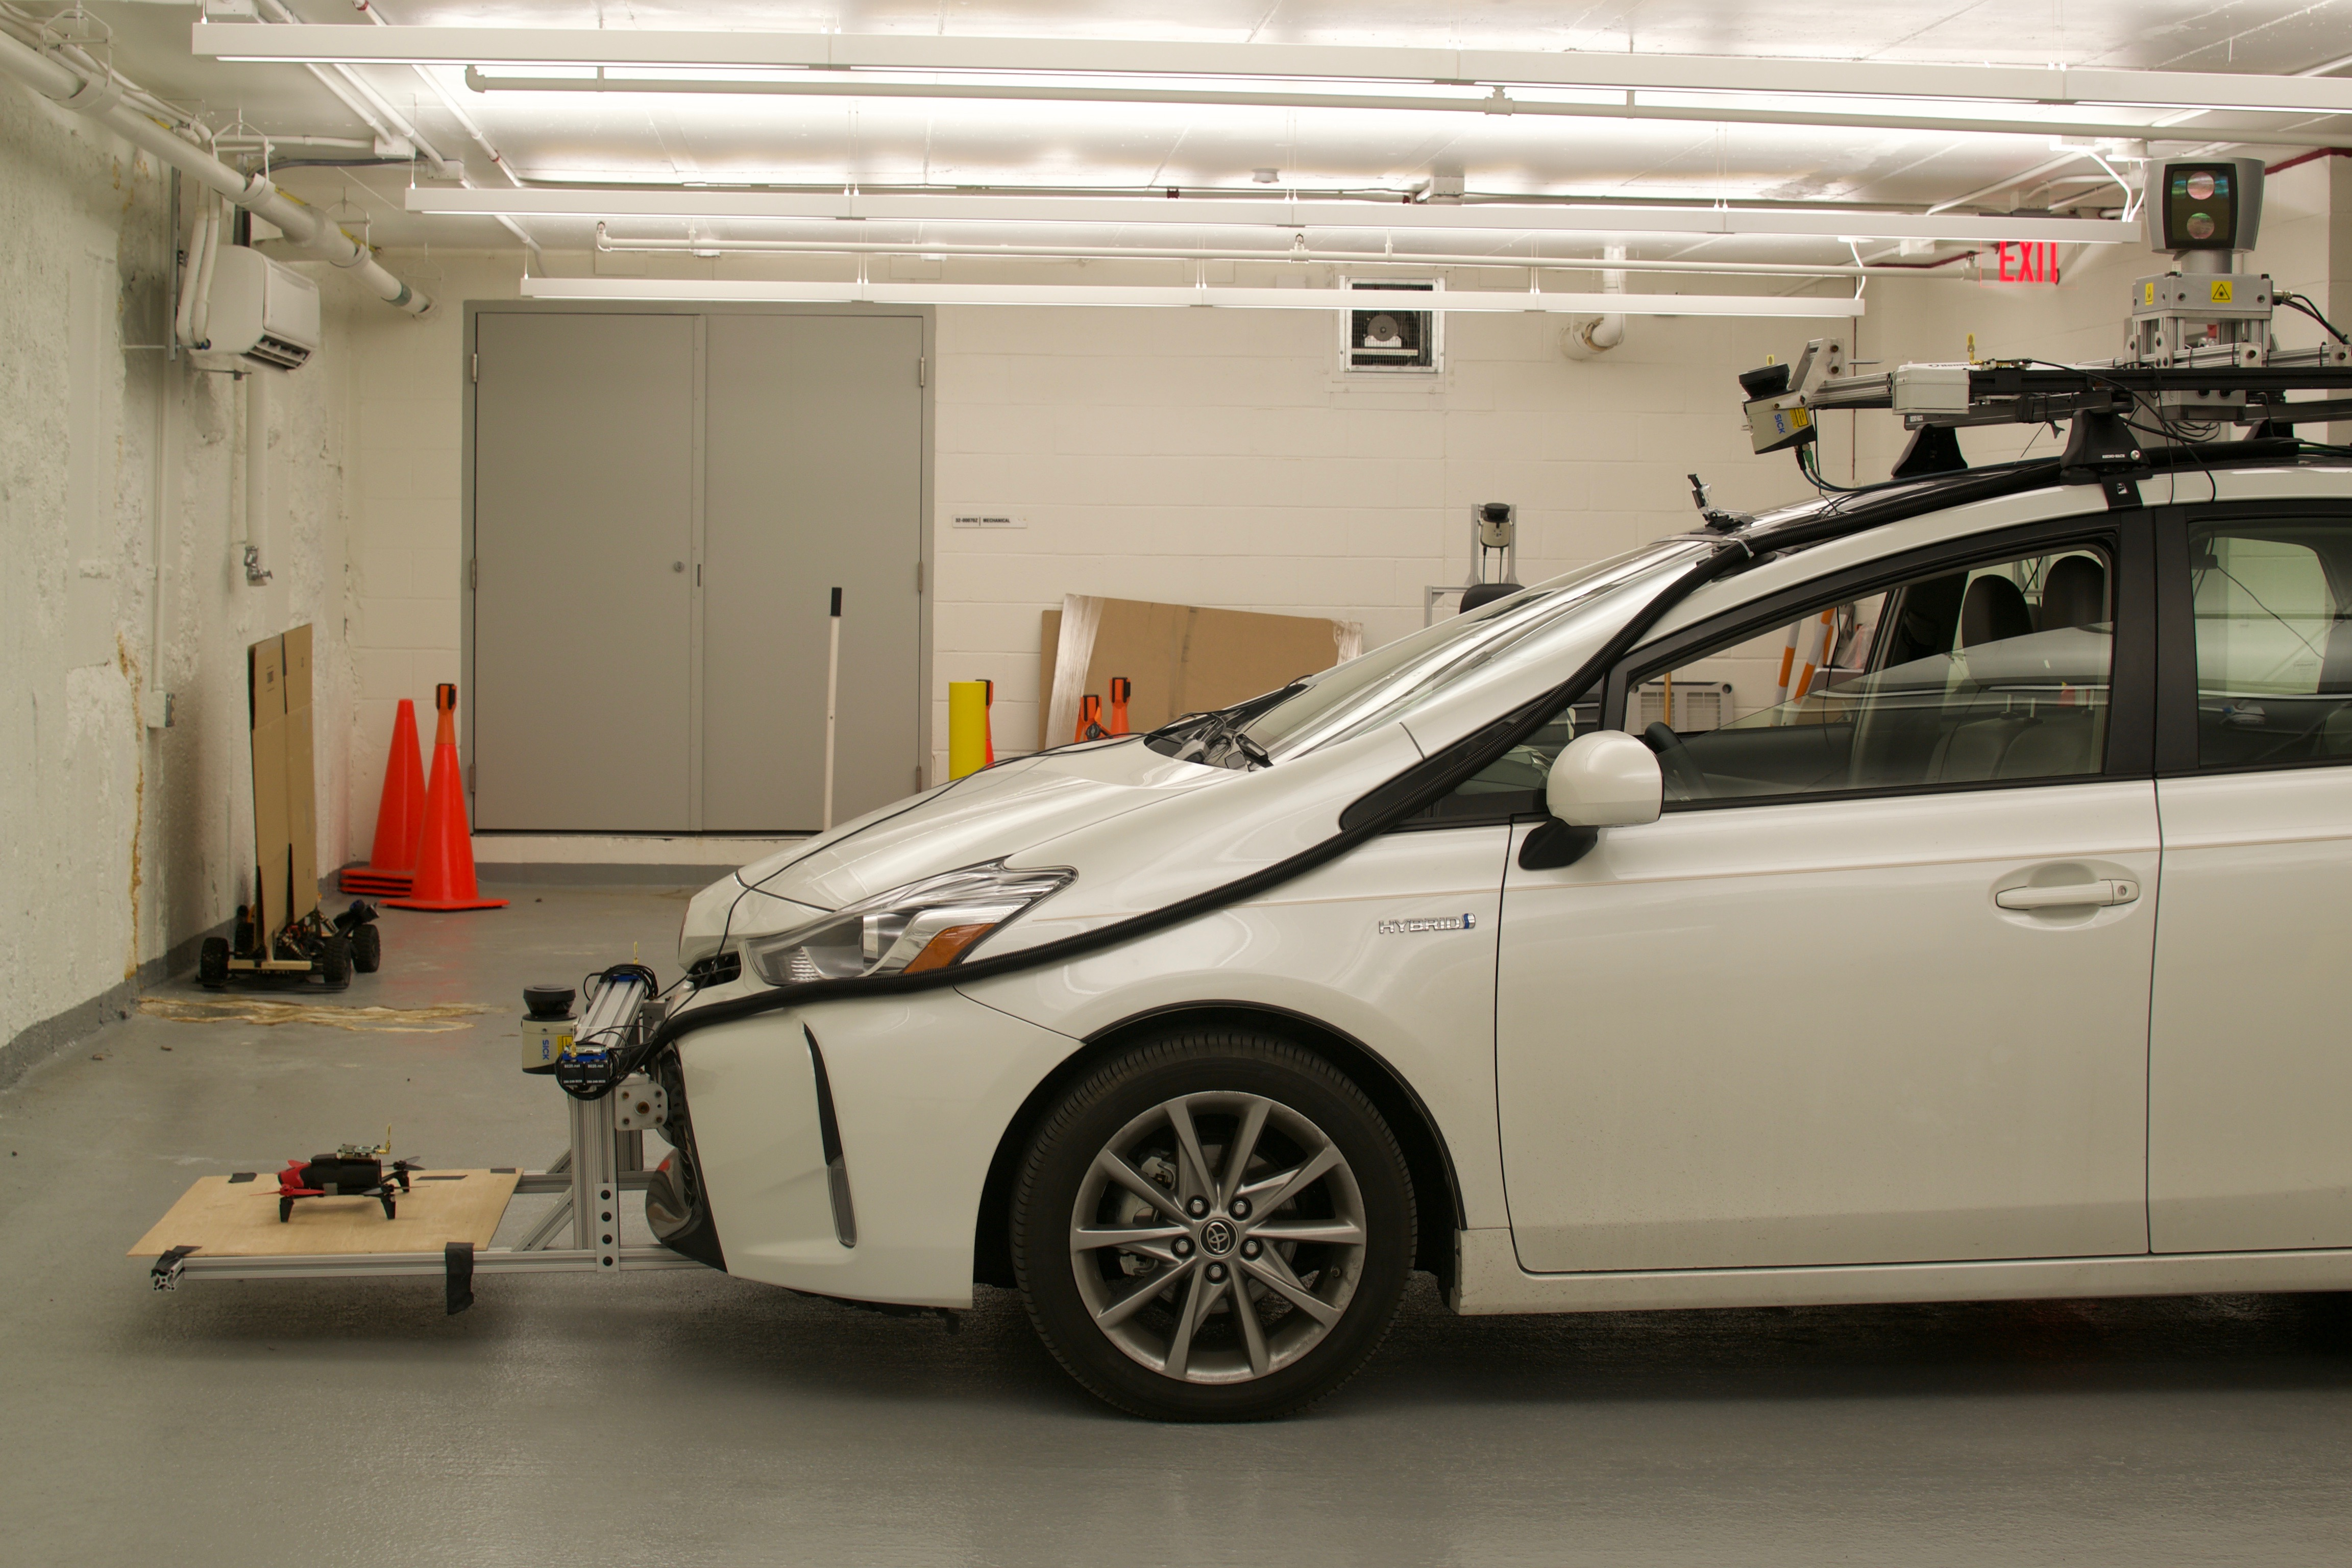
\includegraphics[width=0.49\linewidth]{car-side-view}
    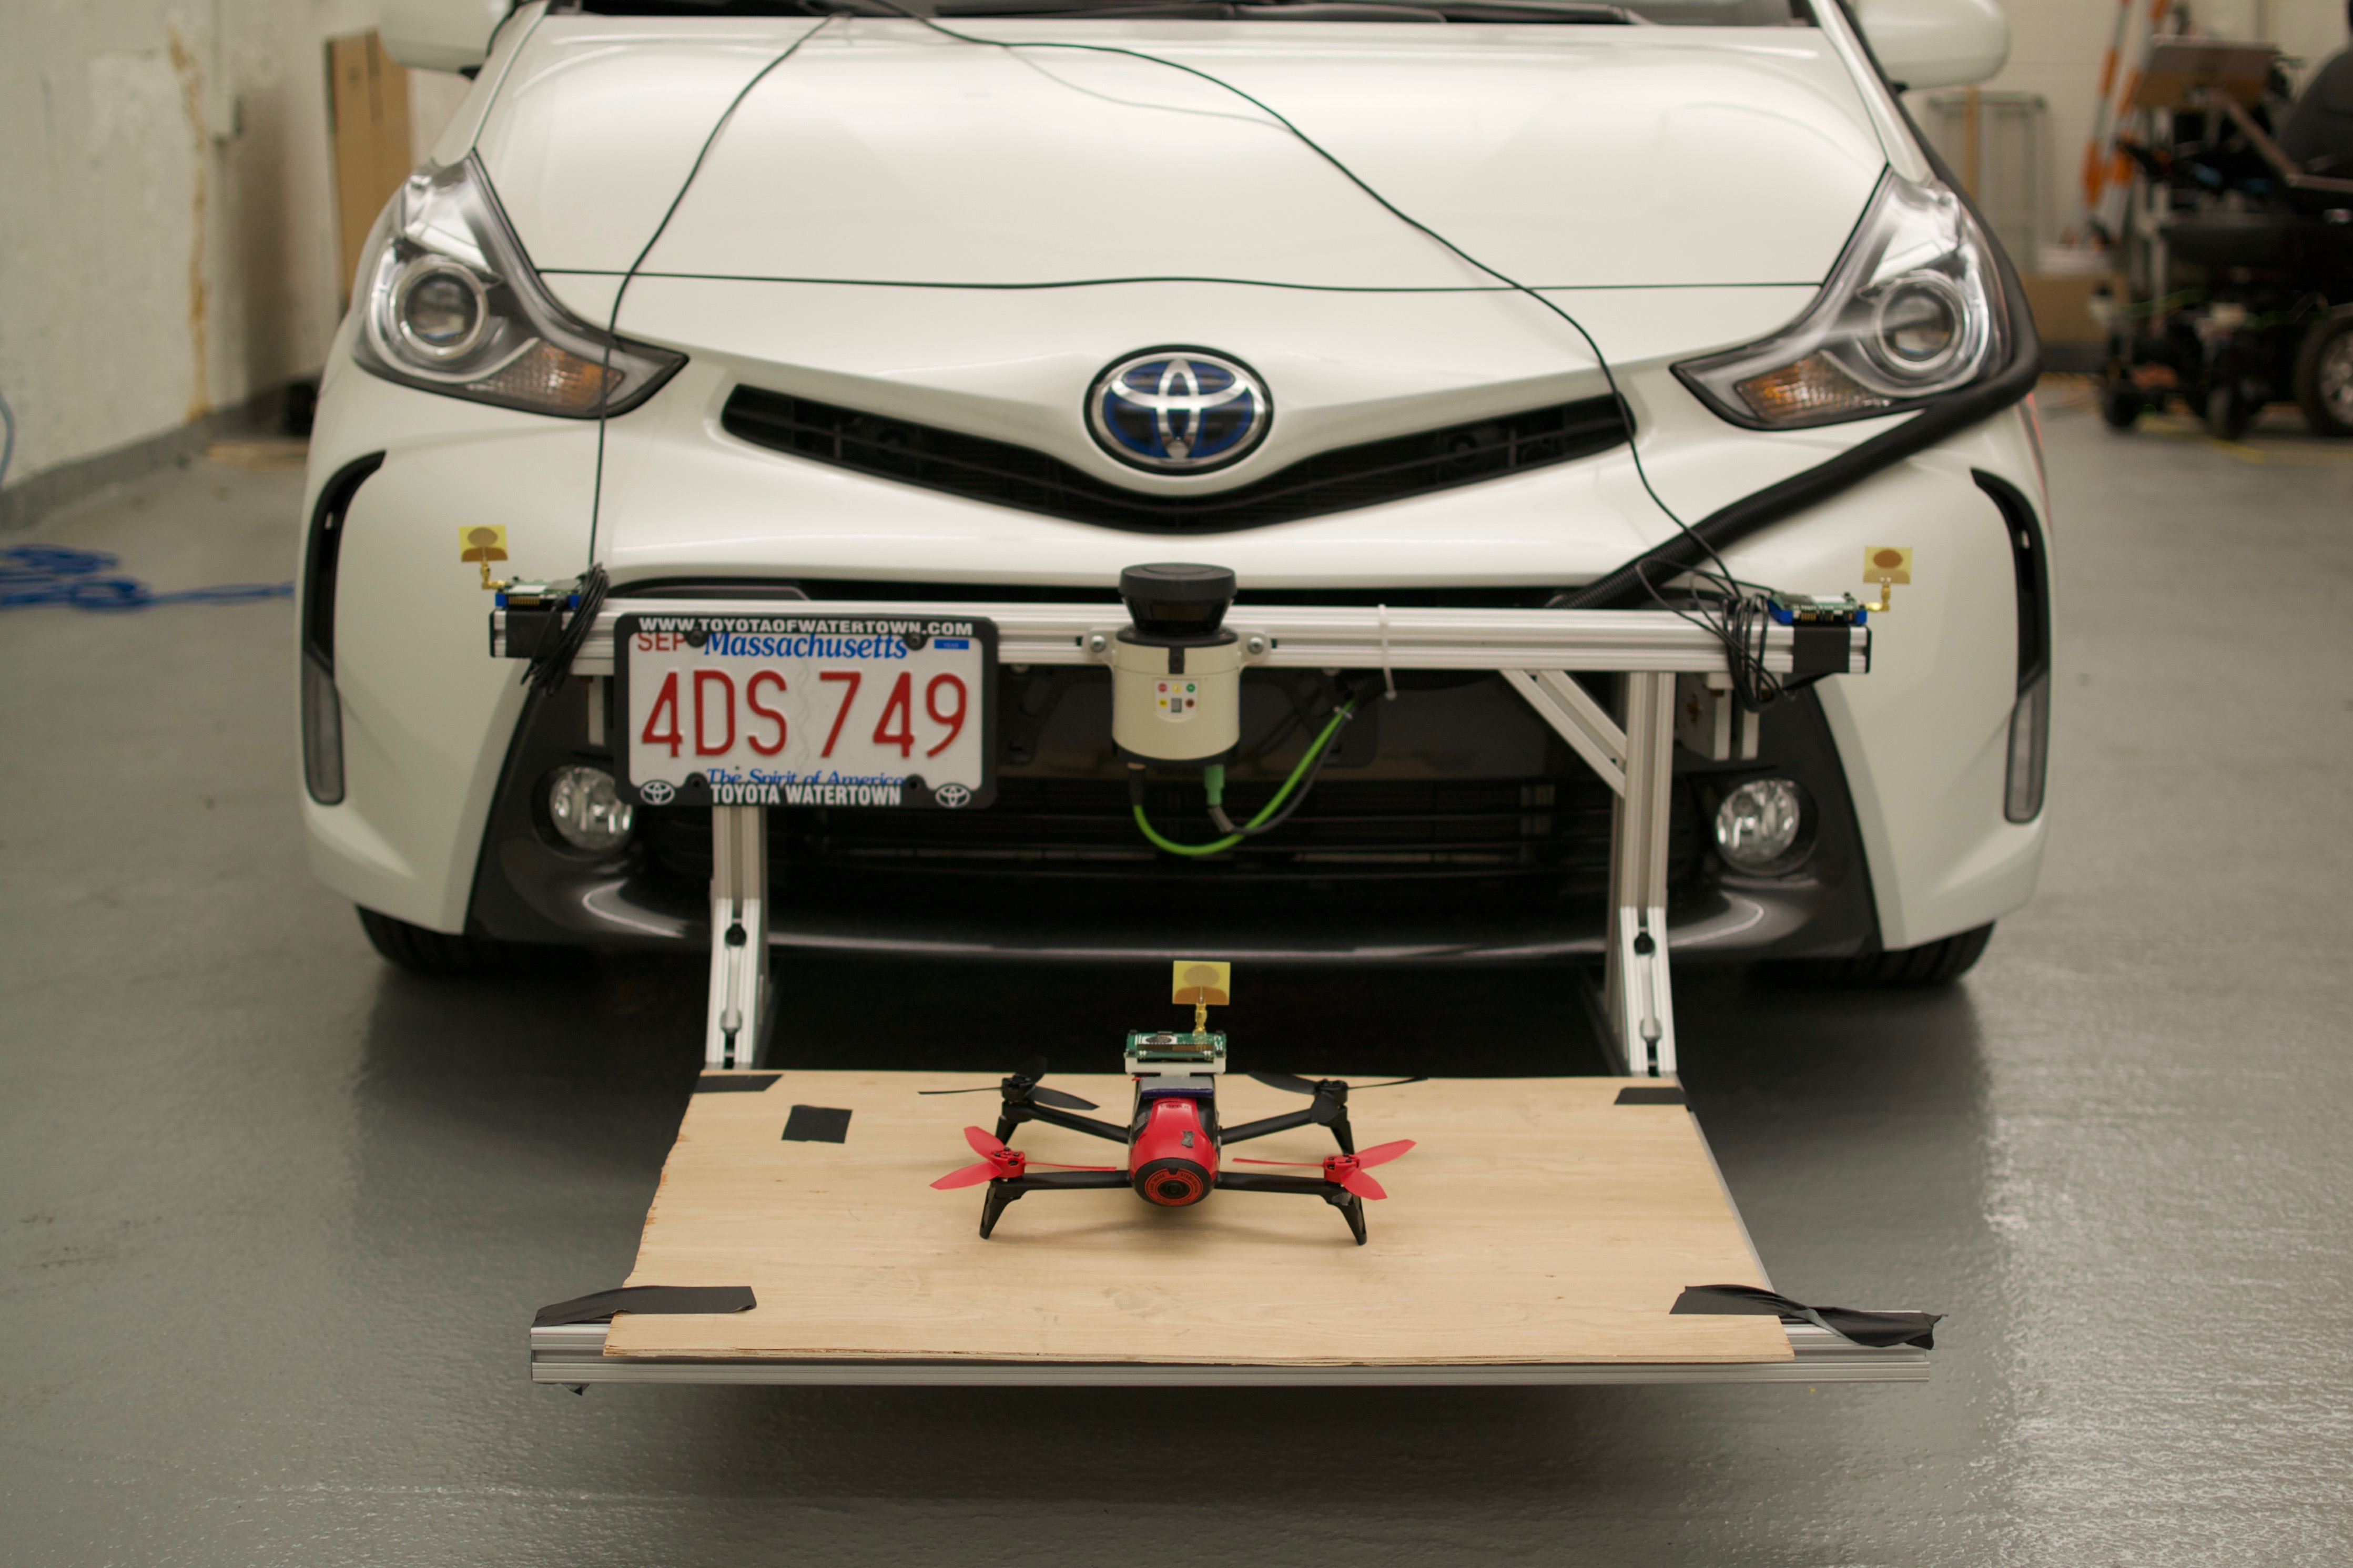
\includegraphics[width=0.49\linewidth]{car-close-up}

    \caption{}

    \label{fig:car}

\end{figure}

We also ran tests using an autonomous golf cart as our ground vehicle in two
different settings.  One setting, shown in Fig.~\ref{fig:exp-buggy-inside}, was
artificially created using tall whiteboards as obstacles to mimic an
adversarial environment. The second, shown in Fig.~\ref{fig:exp-buggy-outside},
was a more realistic setting with the golf cart approaching an open garage door
with blind spots on either side. In both these cases the quadrotor was
successfully able to observe the blind spots and relay this information back to
the computer on board the golf cart. For the interest of brevity, we will only
discuss in detail the experiments using the Toyota Prius.

Our experimental scenario involves a car preparing to leave a garage with a
significant blind spot. The car is unable to sense around the corner to
determine if there are pedestrians or other cars that may obstruct its path.
Our quadrotor takes off from the car's front bumper platform and autonomously
flies out of the garage and looks around the corner. The car is then able to
leave the garage when there are no more pedestrians detected by the quadrotor.
Once the car is ready to return, it backs up into the garage. The quadrotor
then follows the car into the garage and autonomously lands on the platform.

\begin{figure}[t!]

    \centering

    \begin{subfigure}[t]{0.7\textwidth}

        \centering
        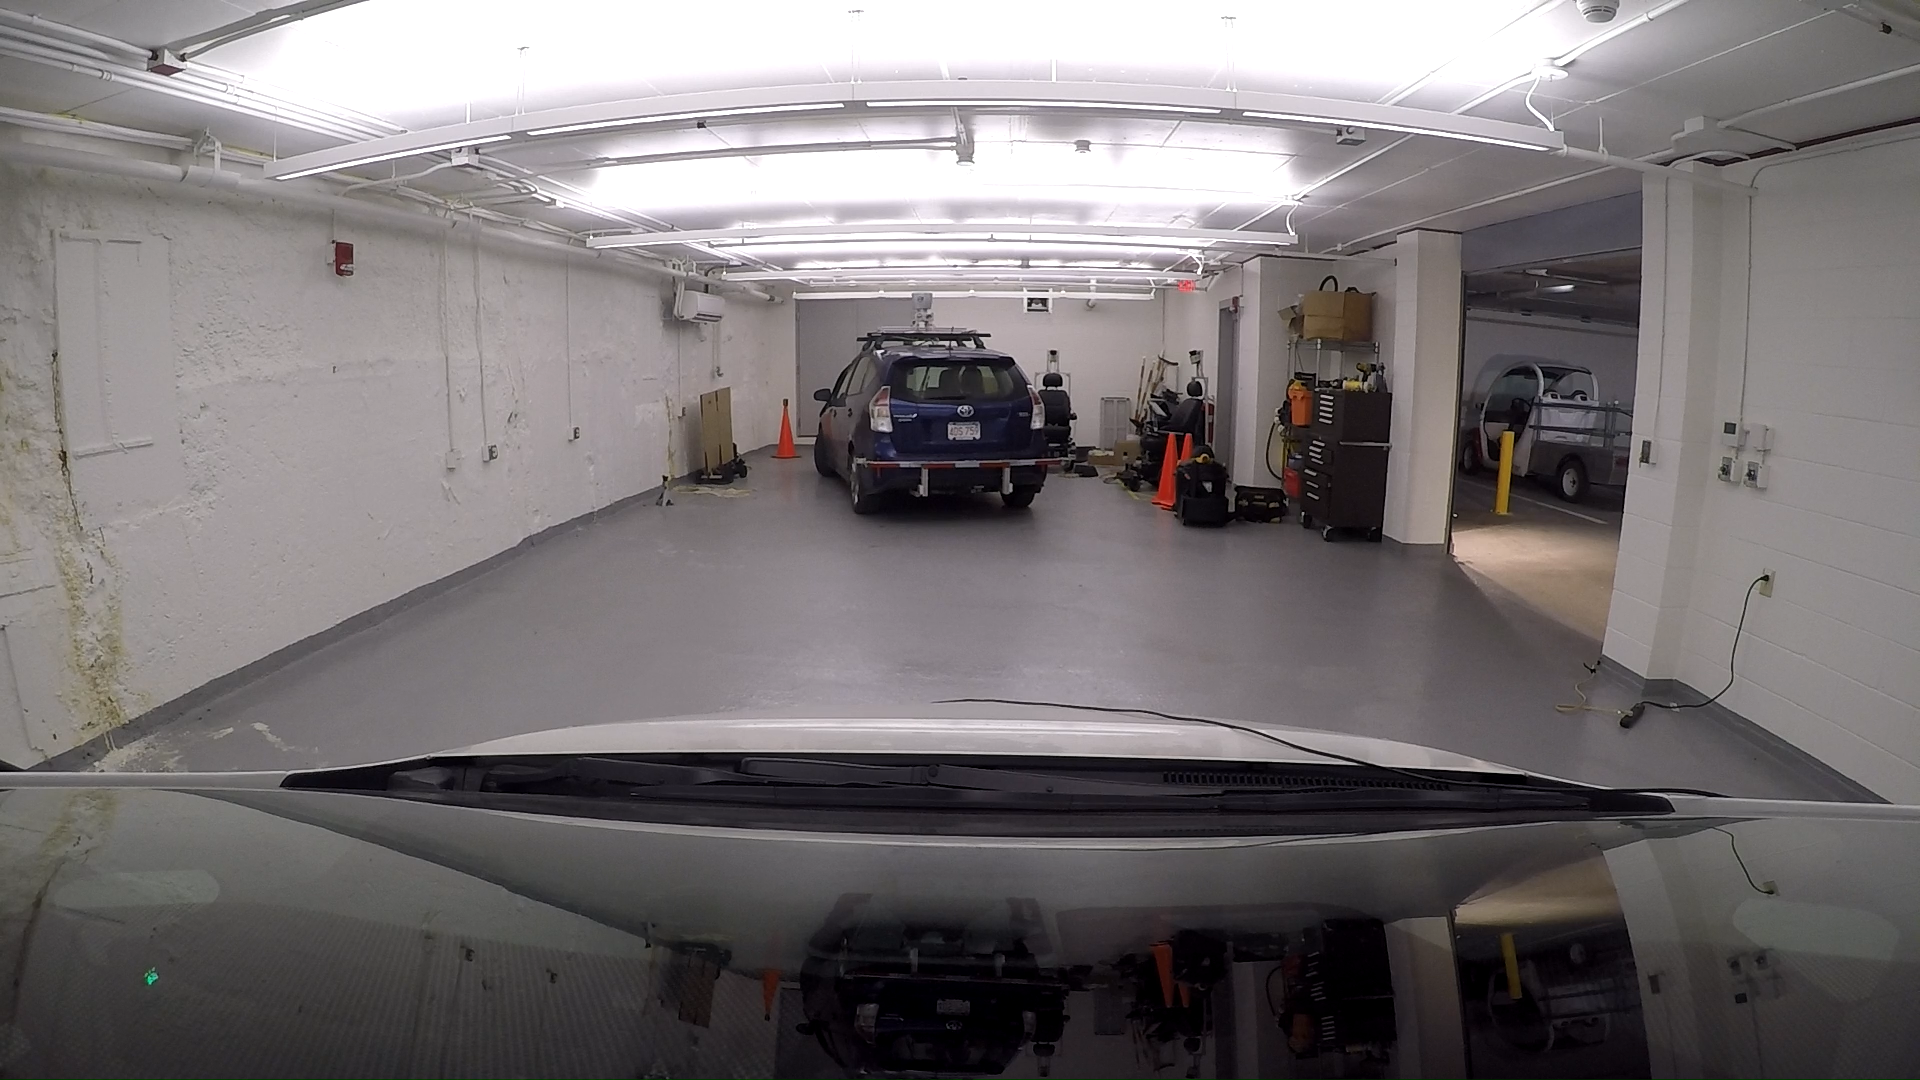
\includegraphics[width=1.0\linewidth]{exp-car-garage}
        \caption{}

        \label{fig:exp-car-garage}

    \end{subfigure}

    \vspace*{1mm}

    \begin{subfigure}[t]{0.7\textwidth}

        \centering
        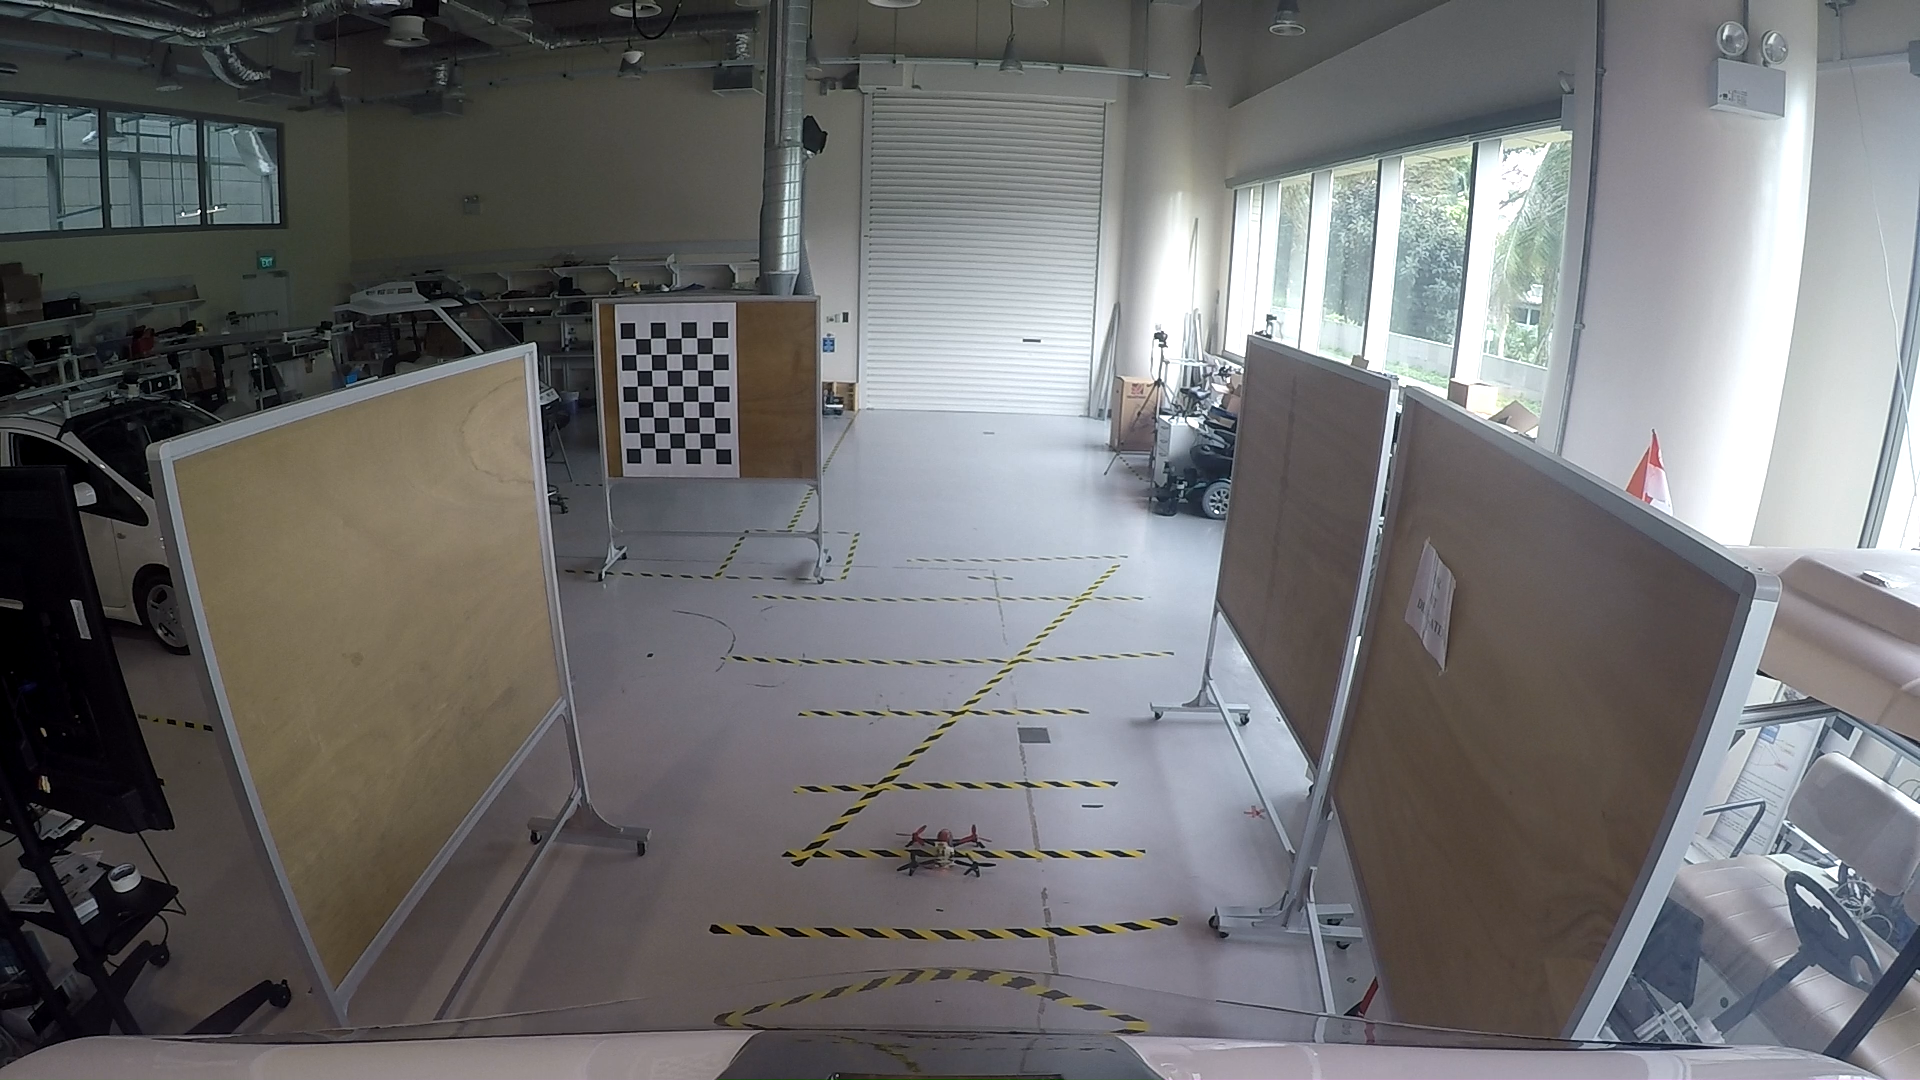
\includegraphics[width=1.0\linewidth]{exp-buggy-inside}
        \caption{}

        \label{fig:exp-buggy-inside}

    \end{subfigure}

    \vspace*{1mm}

    \begin{subfigure}[t]{0.7\textwidth}

        \centering
        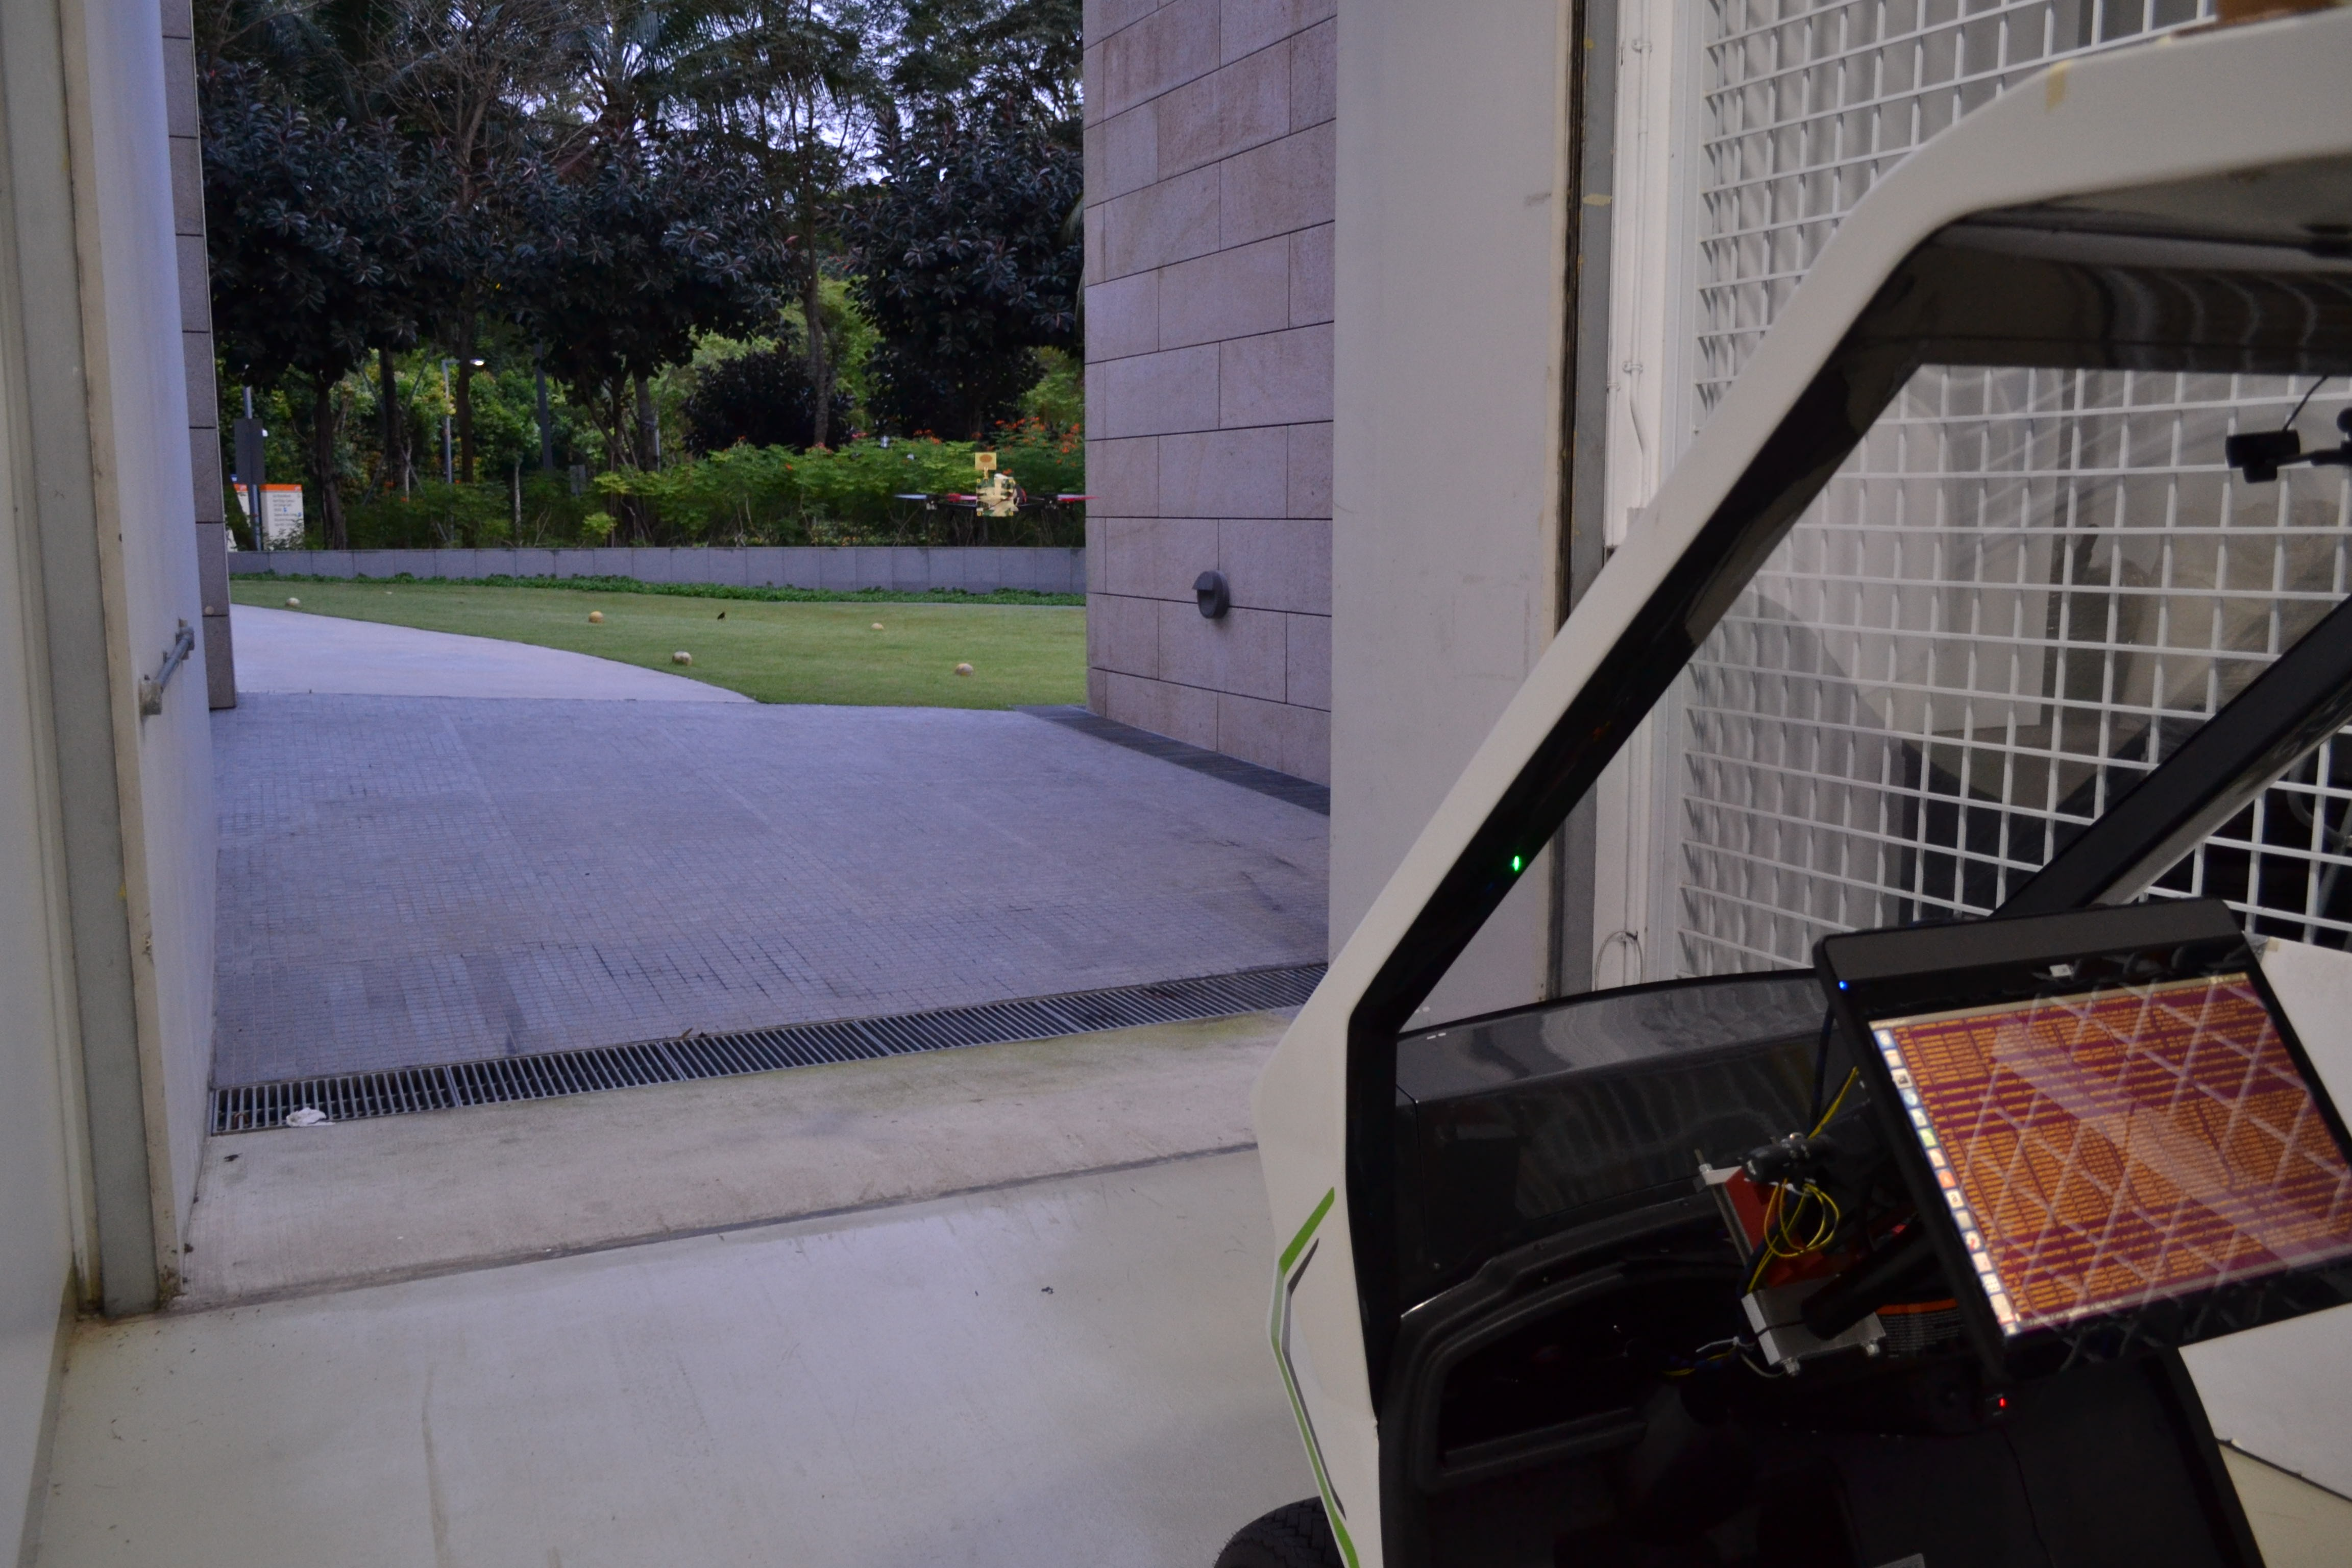
\includegraphics[width=1.0\linewidth]{exp-buggy-outside}
        \caption{}

        \label{fig:exp-buggy-outside}

    \end{subfigure}

    \caption{Snapshots from three different experimental settings we tested our
    algorithm on. Figure (a) used a Toyota Prius. Figures (b) and (c) used an
autonomous golf cart.}

    \label{fig:exps}

\end{figure}

\subsection{Experiment With Quadrotor}

\subsubsection{Looking Around the Corner}

Fig.~\ref{fig:experiment} shows snapshots of the experiment as it progressed.
The first column is a third person angle of the Prius and the quadrotor. The
second column shows frames from the quadrotor's on-board camera along with
object detection and classifications from the convolutional neural net. The
third column is a visualization of the sensor data from the car, the bounding
polygon, blind regions, and the quadrotor's plan. Each row shows a single
snapshot from the experiment.

We can see from the snapshots that the quadrotor is able to successfully take
off from the car, use the laser scan to find the blind regions, and plan a path
to look around the corner in the garage. From the last row, we also see that
our system is able to detect that there is a pedestrian around the corner and
provide the bounding box to the either the driver or an autonomous system
operating the car.

Note that even though the quadrotor is not equipped with the sensors needed to
perform robust 3D obstacle avoidance, it is able to avoid collisions and fly
through the open garage door using the laser scan from the car.

\begin{figure}[h!]

    \centering

    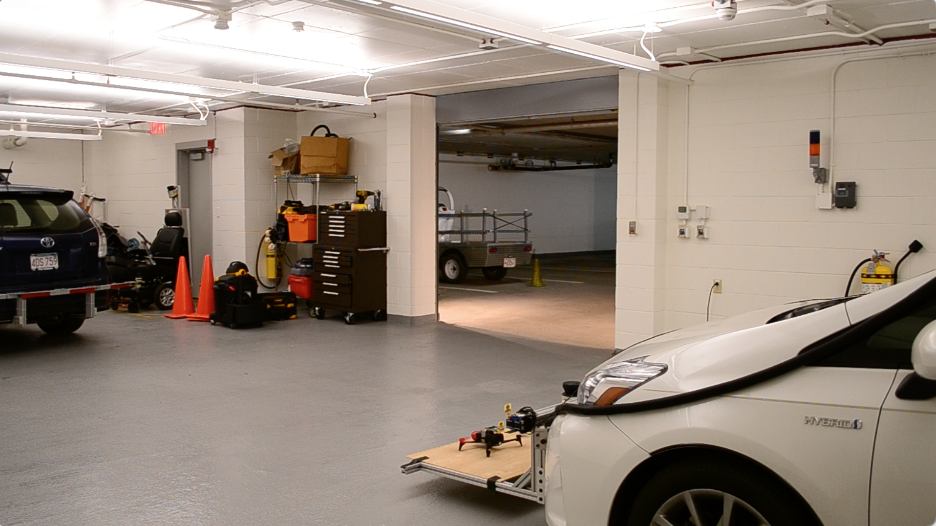
\includegraphics[width=0.35\linewidth]{00-third-person}
    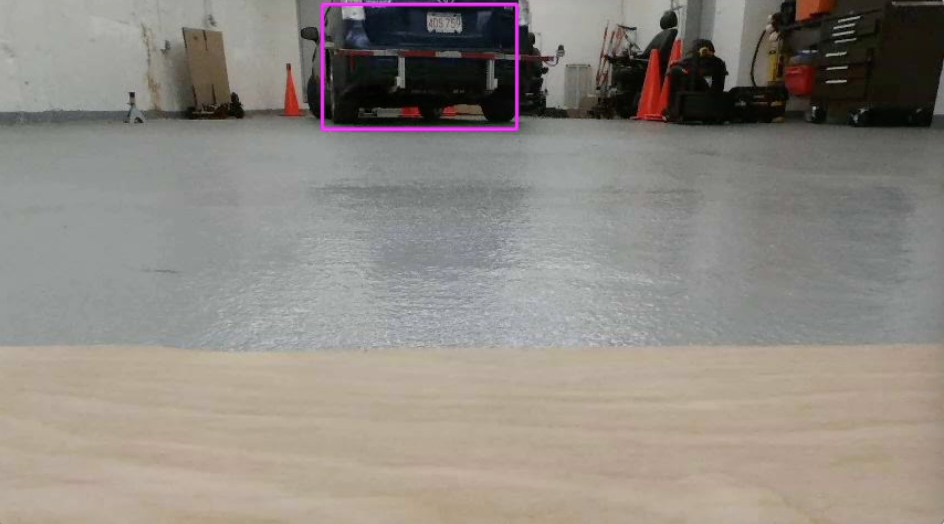
\includegraphics[width=0.35\linewidth]{00-quad-cam}
    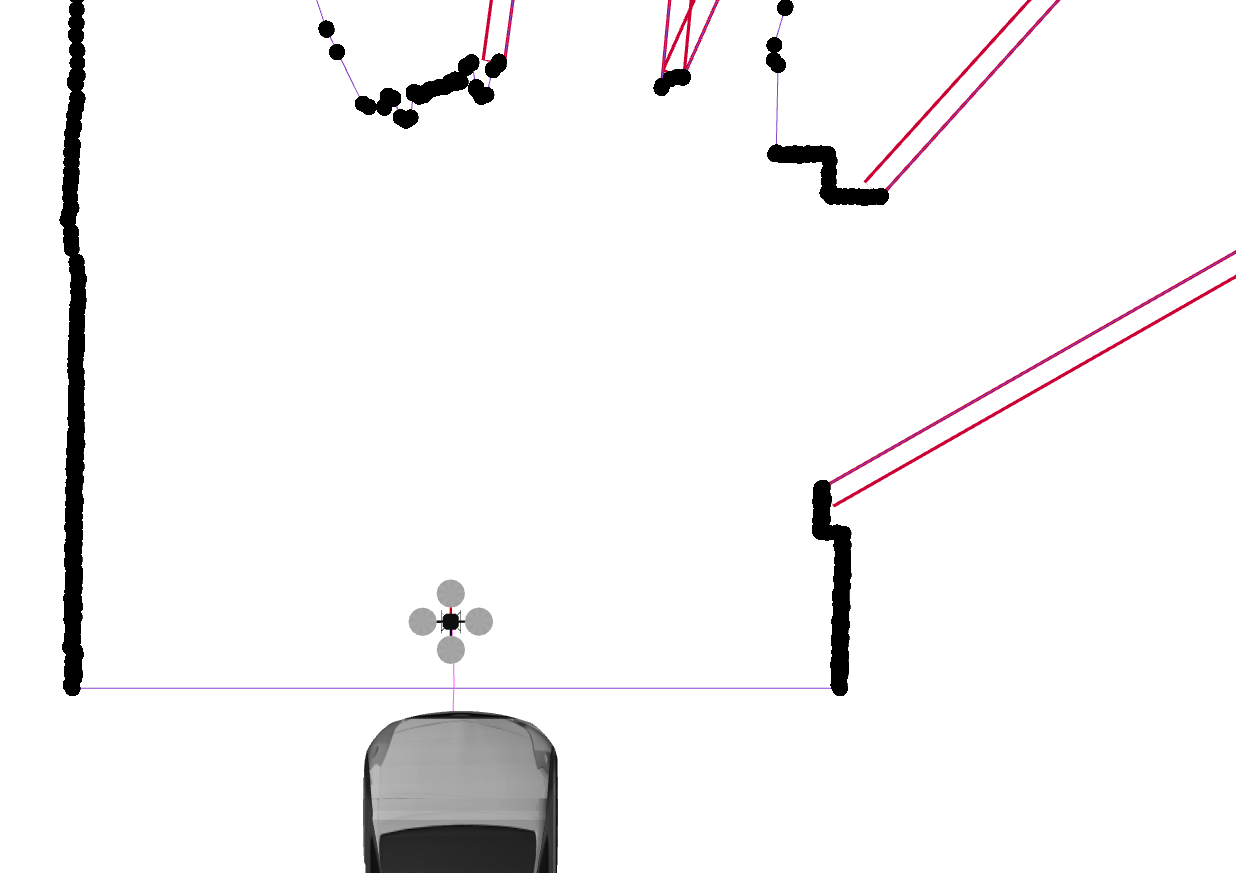
\includegraphics[width=0.28\linewidth]{00-planner-step} \\
    \vspace*{1mm}
    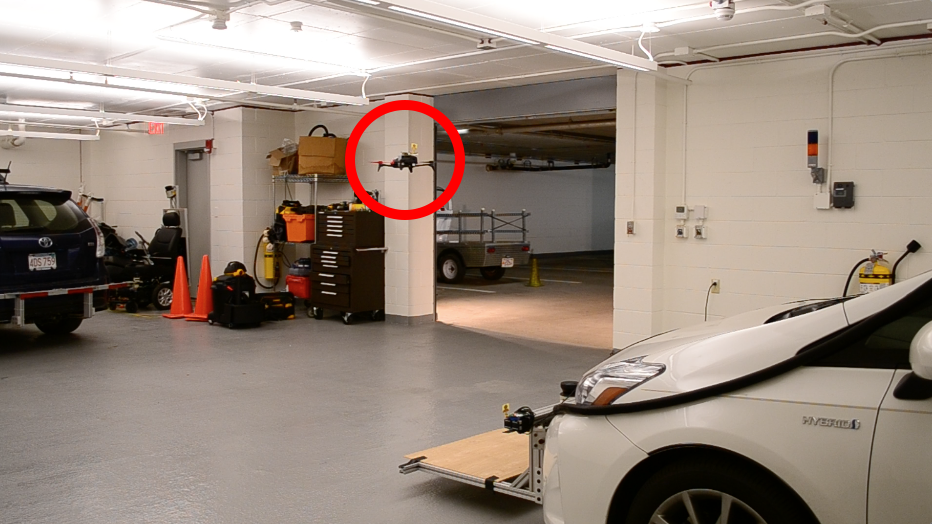
\includegraphics[width=0.35\linewidth]{01-third-person}
    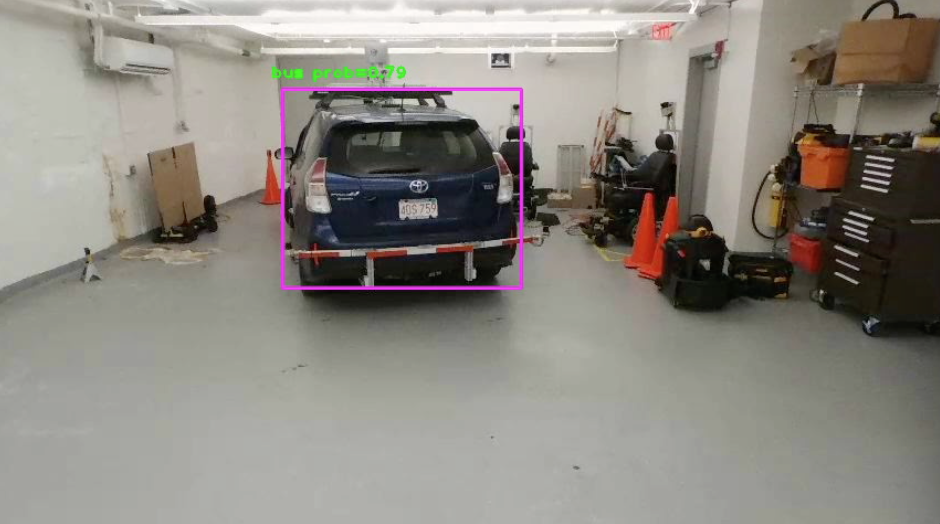
\includegraphics[width=0.35\linewidth]{01-quad-cam}
    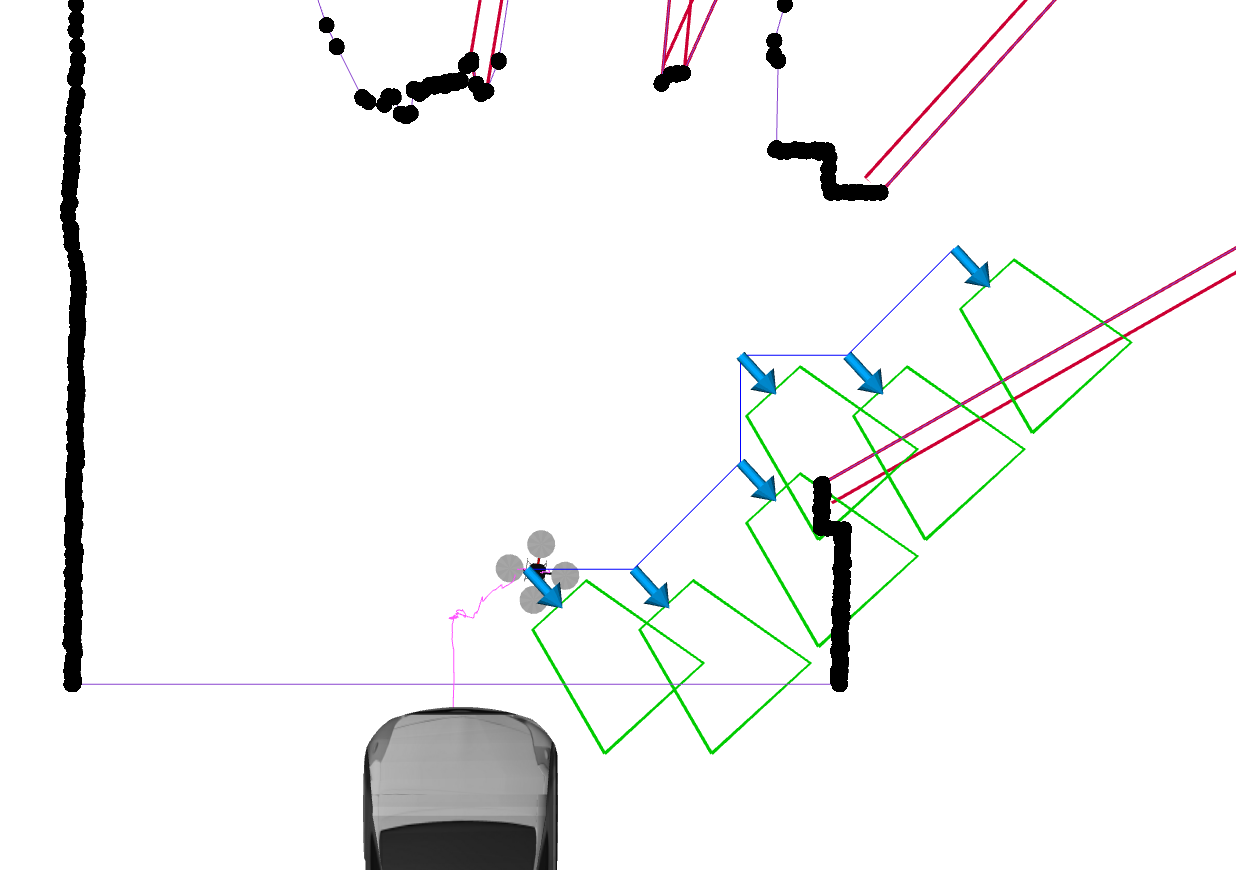
\includegraphics[width=0.28\linewidth]{01-planner-step} \\
    \vspace*{1mm}
    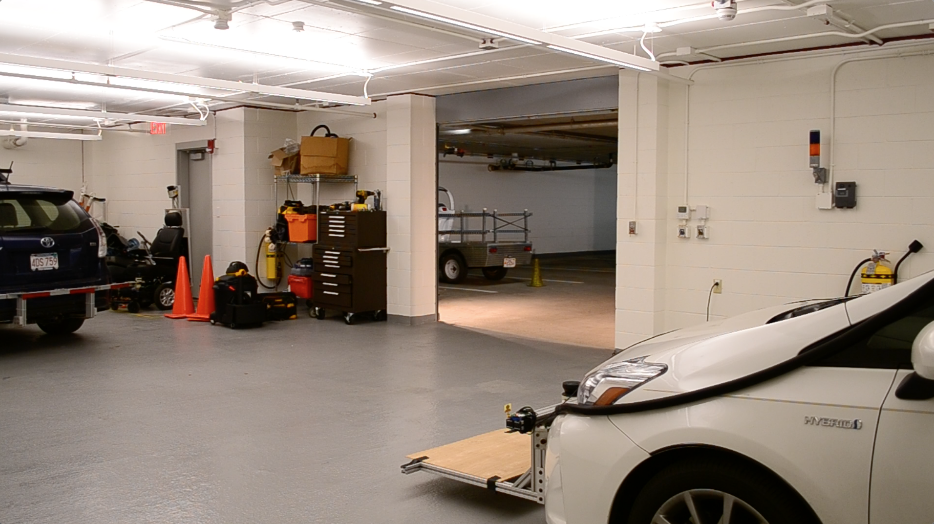
\includegraphics[width=0.35\linewidth]{02-third-person}
    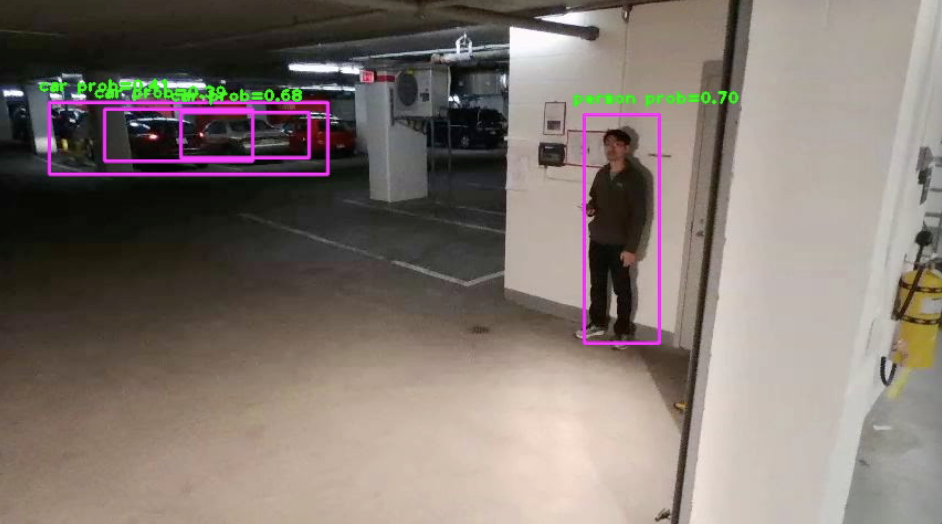
\includegraphics[width=0.35\linewidth]{02-quad-cam}
    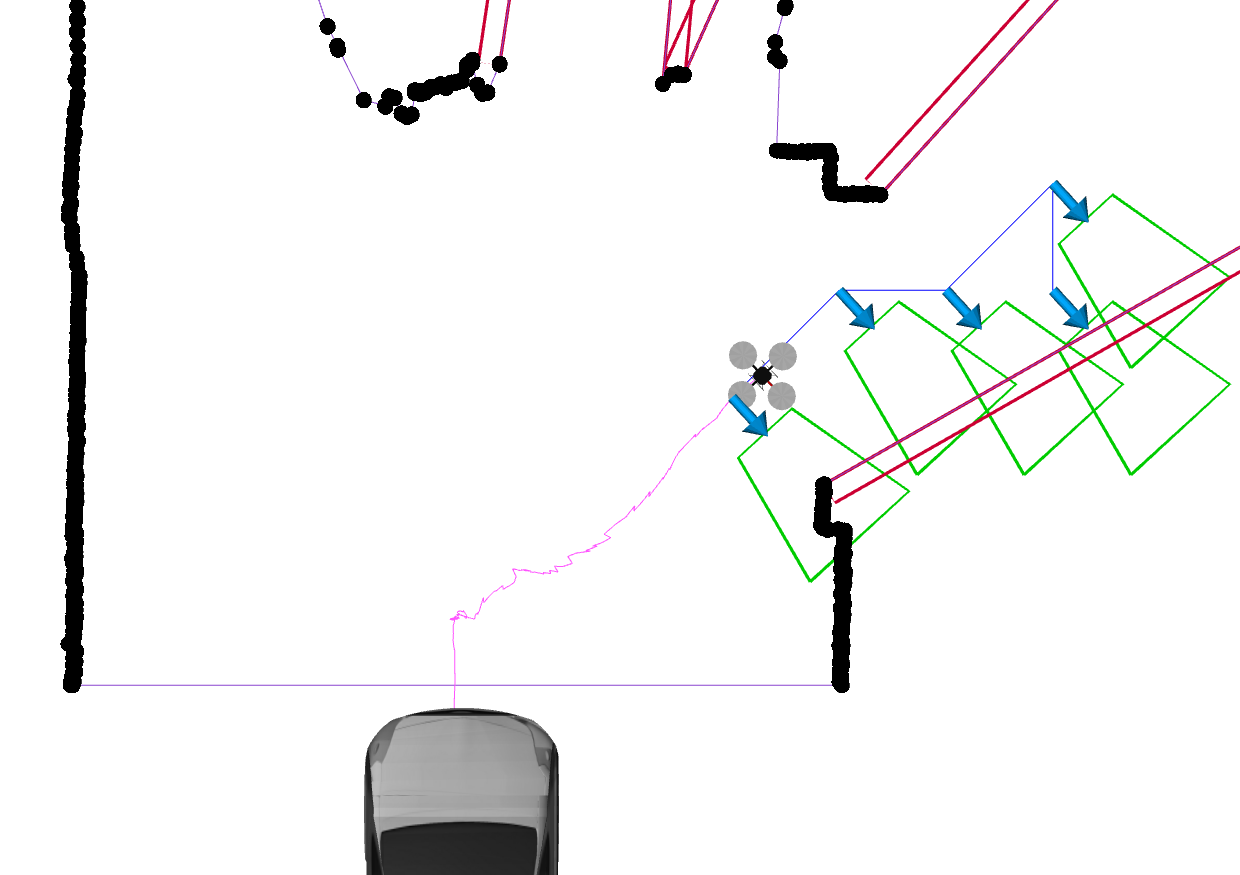
\includegraphics[width=0.28\linewidth]{02-planner-step}

    \caption{}

    \label{fig:experiment}

\end{figure}

\subsubsection{Landing On the Car}

Once the car is ready to park, the quadrotor is able to autonomously land back
on the platform attached to the front bumper. Fig.~\ref{fig:landing}, shows
snapshots from the experiment as the quadrotor followed the car and landed on
the platform. The first image in Fig.~\ref{fig:landing} shows the quadrotor
following the car as it backs up into a garage. The second shows the car parked
and the quadrotor hovering over the platform. The last image shows the
quadrotor after it successfully landed on the platform.

\begin{figure}[h!]

    \centering

    \centerline{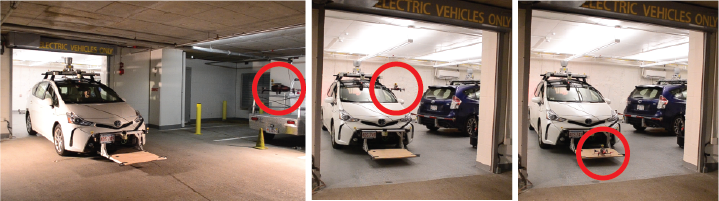
\includegraphics[width=1\linewidth]{landing_sequence}}

    \caption{}

    \label{fig:landing}

\end{figure}


% !TEX root = ../foresight.tex

\section{Conclusion}

In this work we presented a system for using a quadrotor to examine the blindspots of an autonomous car. We developed a path planning algorithm that maximizes visual coverage of blindspots in a 2D laser scan, created an experimental system using UWBs to localize the quadrotor with respect to the car; and performed tests in a variety of environments to verify that our system works. Extensions to our work include planning using 3D laser scan data; improving the accuracy of the UWB localization; and applying our system to other problems such as package delivery and formation control. The authors believe that multi-robot coordination, particularly in the context of an autonomous car and a quadrotor, will find many applications in the future.

\bibliographystyle{spbasic}
\thebibliography{bib}

\end{document}
